\chapter{Metodología}

El desarrollo del trabajo se organiza en cuatro etapas. La primera corresponde a la revisión conceptual de los sistemas HRES-H$_2$ y de las metaheurísticas de población. La segunda implementa un simulador del modelo WPEB y evalúa qué indicadores del artículo de referencia pueden reproducirse bajo los datos supuestos disponibles \cite{Li2024WPEB}. La tercera formula una instancia mixta continua--discreta con un espacio de batería ampliado. La cuarta ejecuta el banco de pruebas comparativo y analiza sus resultados.

Este encadenamiento responde a un principio metodológico explícito: antes de comparar algoritmos se comprueban conservación de energía, límites operacionales y correspondencia cuantitativa con los indicadores publicados. La comparación con Li et al. se denomina reproducción parcial, no demostración absoluta de corrección, porque la ubicación exacta y varios detalles del modelo no fueron publicados.

\section{Herramientas y entorno computacional}

La implementación se desarrolla íntegramente en Python 3.13 dentro de un cuaderno Jupyter autocontenido, \texttt{notebooks/H2\_HRES\_trabajo.ipynb}, compuesto por 68 celdas. El cuaderno y el archivo horario local contienen el modelo, las pruebas, el experimento y las salidas necesarias para reproducir las cifras, sin depender de servicios externos durante la ejecución.

Las bibliotecas empleadas se limitan a cuatro dependencias científicas de uso extendido: \texttt{NumPy} para el álgebra vectorial y la generación de números pseudoaleatorios \cite{Harris2020NumPy}, \texttt{pandas} para la manipulación tabular de resultados \cite{McKinney2010Pandas}, \texttt{matplotlib} para la visualización \cite{Hunter2007Matplotlib} y \texttt{SciPy} para los contrastes estadísticos no paramétricos \cite{Virtanen2020SciPy}. Los algoritmos de optimización se implementan desde cero, sin recurrir a bibliotecas de metaheurísticas de terceros, con el fin de garantizar que los seis competidores comparten exactamente el mismo mecanismo de conteo de evaluaciones, de registro de historial y de interacción con la función objetivo.

\subsection{Decisiones de arquitectura del software}

Varias decisiones de diseño del código son parte sustantiva de la contribución informática del trabajo, en la medida en que son las que hacen auditable el experimento.

\begin{itemize}
    \item \textbf{Configuración inmutable y autovalidada.} Los once bloques de parámetros del escenario se modelan como \textit{dataclasses} con el atributo \texttt{frozen=True} y validación en \texttt{\_\_post\_init\_\_}. Una configuración inconsistente (una eficiencia fuera del intervalo $[0,1]$, una vida útil negativa) falla en el momento de su construcción y no en mitad de una simulación de once minutos. La inmutabilidad garantiza además que ninguna etapa del experimento puede alterar inadvertidamente los parámetros que otra etapa ya empleó.

    \item \textbf{Separación entre instancia y optimizador.} Los seis algoritmos derivan de una clase base \texttt{Optimizer} que fija el contrato de tres métodos: \texttt{\_search} implementa la estrategia de búsqueda propia del algoritmo, \texttt{\_evaluate} contabiliza cada llamada a la función objetivo y \texttt{\_record} registra el historial de convergencia. Un registro de algoritmos permite añadir un competidor nuevo sin tocar el código de ejecución del banco de pruebas. Esta separación es la que hace posible garantizar el presupuesto idéntico de evaluaciones.

    \item \textbf{Memoización de perfiles de generación.} Los perfiles horarios eólico y fotovoltaico dependen únicamente de la capacidad instalada. Una memoria intermedia indexada por capacidad evita recalcular 8.760 valores cuando reaparece una capacidad ya evaluada. Las solicitudes repetidas cuentan igualmente contra el presupuesto y se informan por separado.

    \item \textbf{Ejecución a dos escalas.} Un único interruptor de configuración alterna entre un modo rápido (3 semillas, 8 individuos y 8 iteraciones) y el modo completo empleado para los resultados definitivos (30 semillas, 20 individuos y 30 iteraciones). El primero permite verificar el flujo de extremo a extremo antes de ejecutar el presupuesto definitivo.

    \item \textbf{Tipos explícitos para el dominio.} Las políticas de despacho se modelan como enumeraciones y los diseños y resultados como estructuras con campos nombrados, de modo que las decisiones del modelo quedan expresadas en el sistema de tipos y no en constantes numéricas dispersas por el código.
\end{itemize}

\section{Fuente de datos y horizonte temporal}

Los datos meteorológicos proceden de NASA POWER \cite{NasaPower}, para las coordenadas aproximadas de Damao Banner, Baotou, Mongolia Interior (latitud 41,70; longitud 110,43), en la zona horaria UTC+8. El artículo de referencia no publica las coordenadas exactas del emplazamiento, limitación que se discute entre los supuestos del trabajo.

La serie se almacena localmente en \texttt{notebooks/src/hourly\_2008.csv} y contiene cuatro columnas: velocidad de viento a 50 m (\texttt{ws50m}), velocidad de viento extrapolada a altura de buje (\texttt{wsc\_ms}), irradiancia global horizontal (\texttt{ghi\_kwh\_m2}) y temperatura del aire a 2 m (\texttt{t2m\_c}). El archivo \texttt{notebooks/src/data\_provenance.csv} registra coordenadas, horizonte, resolución y columnas. La versión del producto o de la API no fue conservada en el artefacto original y se declara como ``no registrada''; esta omisión limita la reproducción externa y no se completa retrospectivamente con una versión actual. El almacenamiento local garantiza, en cambio, que las ejecuciones de esta tesis operen sobre los mismos valores.

El año de análisis es 2008, seleccionado por consistencia con el artículo. Aunque es bisiesto, Li et al. declara reiteradamente una serie de 8.760 horas \cite{Li2024WPEB}. La reproducción principal elimina exactamente las 24 marcas del 29 de febrero, sin interpolación. La serie íntegra de 8.784 horas se conserva y se ejecuta como sensibilidad separada.

\begin{figure}[H]
\centering
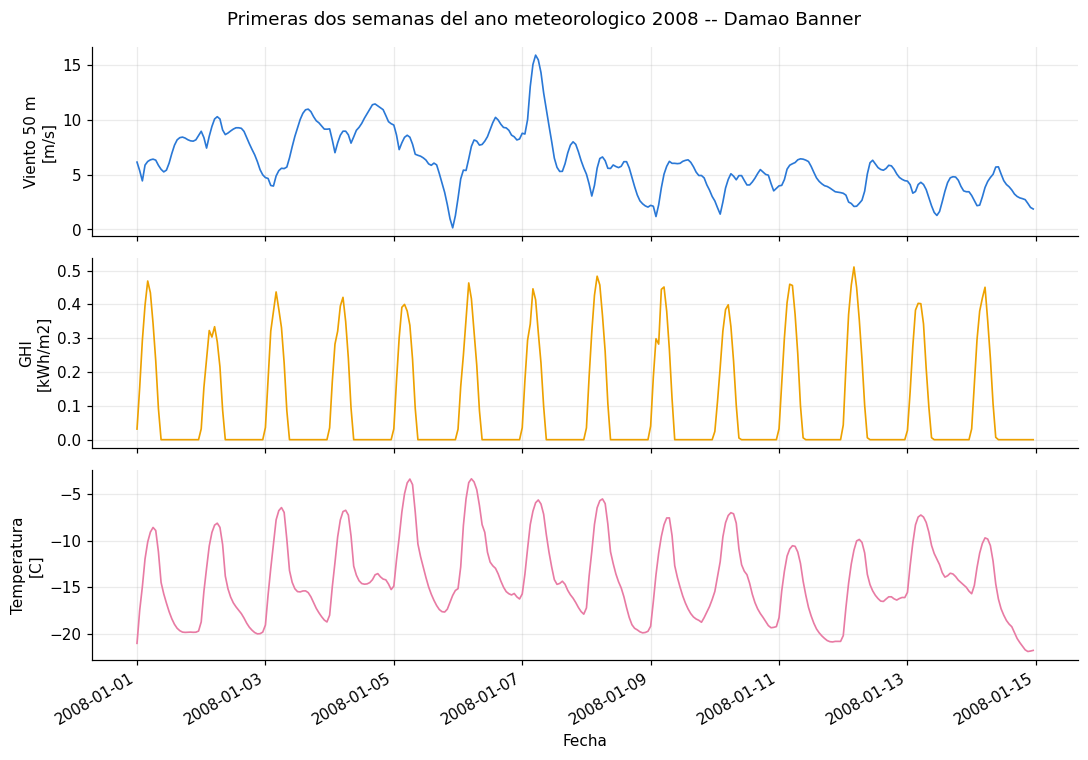
\includegraphics[width=0.92\textwidth]{figures/fig01_recurso_meteorologico.png}
\caption{Recurso meteorológico durante las dos primeras semanas del año 2008 en Damao Banner: velocidad de viento a 50 m, irradiancia global horizontal y temperatura ambiente.}
\label{fig:recurso}
\end{figure}

En el horizonte principal, el recurso reconstruido presenta una velocidad media a 50 m de 7,09 m/s y una irradiancia global horizontal acumulada de 1.658 kWh/m$^2$. Li et al. informa 7,56 m/s y 1.731 kWh/m$^2$; esta diferencia objetiva limita la reproducibilidad del caso antes de aplicar cualquier modelo de conversión.

\section{Decisiones de modelado justificadas por evidencia}
\label{sec:decisiones_modelado}

Tres decisiones del modelo se apartan de la lectura literal del artículo de referencia o resuelven ambigüedades que este deja abiertas. Se documentan aquí de forma explícita porque afectan a los resultados y porque su justificación es empírica y no de conveniencia.

\subsection{Selección de la serie de velocidad de viento}

El artículo declara una altura de buje de 105 m, pero no publica la curva de potencia real, las pérdidas de estela ni otros descuentos necesarios para reconstruir el parque. La serie a 50 m define el escenario principal y la extrapolación a 105 m se evalúa como sensibilidad. No se selecciona una de ellas por su cercanía posterior al LCOE publicado. Por tanto, una diferencia observada no permite concluir qué transformación aplicaron los autores.

\subsection{Corrección de la interpretación de la irradiancia}

Una versión anterior de la implementación interpretaba la irradiancia global horizontal en unidades incompatibles con el modelo térmico de la celda fotovoltaica, lo que producía temperaturas de celda físicamente imposibles y, como consecuencia, una producción fotovoltaica prácticamente nula: el factor de capacidad resultante era del 0,72\,\% frente al 19\,\% publicado. Corregida la interpretación, el factor de capacidad fotovoltaico pasa a 0,1874, con un desvío del $-1{,}34\,\%$.

El episodio se consigna por su valor metodológico. El error no producía excepciones ni resultados manifiestamente absurdos en las magnitudes agregadas: el simulador entregaba costos nivelados plausibles, y solo el contraste sistemático contra indicadores publicados permitió detectarlo. Es un argumento a favor de la verificación cuantitativa frente a la mera inspección de que el código «funciona».

\subsection{Reparto del costo de la batería entre potencia y energía}

El artículo de referencia expresa el costo de la batería exclusivamente por unidad de potencia instalada, imputación coherente con su modelo porque en él la duración está fijada en una hora y potencia y energía resultan numéricamente equivalentes. Al convertir la duración en variable de decisión, esa imputación deja de ser válida: alargar la batería de una a cuatro horas sería gratuito, y la variable carecería de contenido económico.

Se adopta por ello un reparto del costo entre una componente por potencia (30\,\%) y otra por energía (70\,\%), definido de modo que la suma reproduzca el costo original para una duración de una hora. Es una extensión económica introducida por esta tesis, no un parámetro publicado por Li et al.

\begin{table}[H]
\centering
\footnotesize
\caption{Reparto del costo de la batería entre componentes de potencia y de energía}
\label{tab:reparto_bateria}
\renewcommand{\arraystretch}{1.2}
\begin{tabular}{l r r r}
\hline
\textbf{Concepto} & \textbf{Por potencia} & \textbf{Por energía} & \textbf{Suma a 1 h} \\
 & \textbf{[CNY/kW]} & \textbf{[CNY/kWh]} & \textbf{[CNY/kW]} \\
\hline
Inversión inicial & 764{,}70 & 1784{,}30 & 2549{,}00 \\
Reemplazo & 150{,}00 & 350{,}00 & 500{,}00 \\
Operación y mantenimiento anual & 3{,}00 & 7{,}00 & 10{,}00 \\
\hline
\end{tabular}
\end{table}

\section{Modelos de generación y validación del recurso}

La generación eólica se calcula con una curva de potencia cúbica por tramos expresada por unidad de MW y escalada por la capacidad agregada continua $W$. No se redondea el número de turbinas ni se aplica un recorte posterior dependiente de ese redondeo. La generación fotovoltaica aplica un modelo de temperatura de celda basado en la temperatura nominal de operación, con corrección por coeficiente térmico, factor de pérdidas, sobredimensionamiento del generador respecto del inversor y recorte a la potencia nominal de este último.

\begin{figure}[H]
\centering
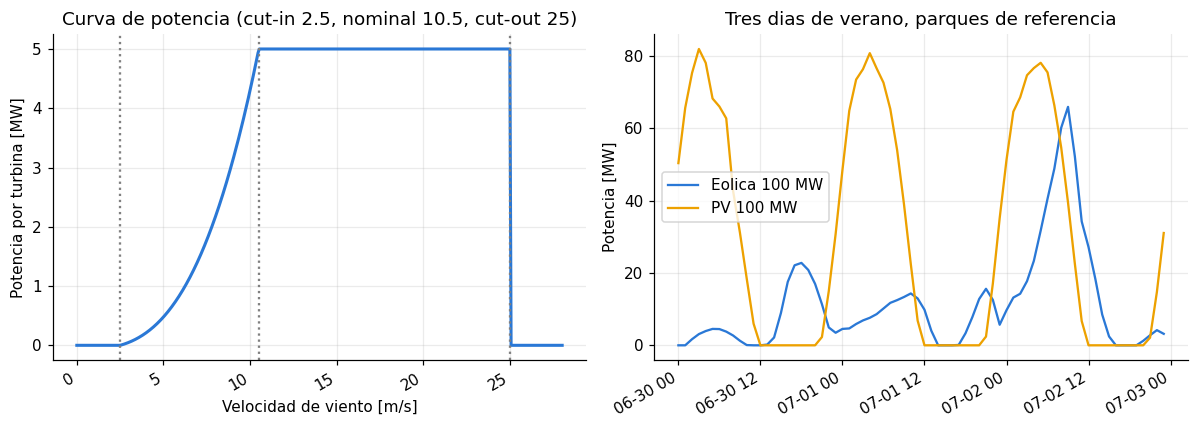
\includegraphics[width=\textwidth]{figures/fig02_curva_potencia_generacion.png}
\caption{Izquierda: curva de potencia de la turbina de 5 MW, con las velocidades de arranque, nominal y de corte. Derecha: perfiles de generación eólica y fotovoltaica de 100 MW durante tres días de verano, donde se aprecia la complementariedad temporal entre ambos recursos.}
\label{fig:generacion}
\end{figure}

La Figura~\ref{fig:generacion} ilustra la complementariedad que justifica la hibridación: la generación fotovoltaica se concentra en las horas centrales del día, mientras que la eólica presenta una distribución más uniforme y con frecuencia máximos nocturnos. Es esta complementariedad la que permite sostener el electrolizador por encima de su carga mínima durante una fracción mayor del año que la alcanzable con cualquiera de los dos recursos por separado.

\section{Modelo económico}

La evaluación económica sigue la estructura de costo presente neto habitual en el dimensionamiento de microrredes \cite{Lambert2006Homer}. Para cada componente se suman la inversión inicial, el valor presente de los reemplazos que correspondan dentro del horizonte de 25 años y el valor presente de los costos anuales de operación y mantenimiento, descontando el valor residual del componente al término del proyecto mediante depreciación lineal sobre la vida útil restante. Con una tasa de descuento real del 4,35\,\% y un horizonte de 25 años, el factor de recuperación de capital resulta de 0,066402.

El electrolizador, con una vida útil de 15 años, incorpora un reemplazo en el año 15; la batería, con una vida útil de 10 años, incorpora reemplazos en los años 10 y 20. El almacenamiento de hidrógeno se dimensiona en 10.000 kg fijos e ingresa al costo presente neto con su inversión y su operación, sin reemplazo ni valor residual por coincidir su vida útil con el horizonte del proyecto.

El costo anualizado se obtiene multiplicando el costo presente neto por el factor de recuperación de capital. El costo nivelado de la energía divide ese costo anualizado por la energía útil anual, definida como la suma de la energía entregada al electrolizador y la vendida a la red. El $\mathrm{LCOH}_{\mathrm{tesis}}$ divide el mismo costo anualizado por la producción anual de hidrógeno; es un indicador secundario con la asignación de costos propia ya declarada.

\section{Simulación horaria y despacho}

Cada configuración candidata se evalúa mediante una simulación secuencial de las 8.760 horas del horizonte principal. El estado de carga de la batería en cada hora depende del estado precedente; por ello el despacho se calcula cronológicamente. La sensibilidad de 8.784 horas ejecuta el mismo algoritmo sin retirar el 29 de febrero.

El despacho horario aplica una prioridad fija sobre la energía renovable disponible: primero alimentar el electrolizador, después cargar la batería con el excedente, a continuación exportar a la red y, finalmente, verter el remanente que exceda la capacidad de conexión. El modelo no permite compras de electricidad a la red; $P_{grid,t}$ representa solo exportación no negativa. La carga auxiliar de planta se fija en cero porque su magnitud no está publicada, mientras que las eficiencias del rectificador y del convertidor bidireccional se aplican explícitamente. Las dos políticas de gestión de la carga mínima del electrolizador, que constituyen una de las diferencias entre las dos instancias de optimización, se detallan en el capítulo de diseño experimental.

Concluida la simulación, se calculan los agregados anuales, se verifica la restricción sobre la fracción de energía vendida a la red y se evalúan los indicadores económicos. Cuando una configuración incumple una restricción verificable antes de simular, la función de evaluación retorna un resultado infactible acompañado del motivo textual del rechazo, lo que facilita la depuración y permite auditar por qué una región del dominio quedó excluida.

\section{Parámetros del escenario}

Las Tablas~\ref{tab:parametros_configuracion_replica}--\ref{tab:parametros_costos_conversion_replica} recogen los parámetros empleados. Se usan los valores publicados por Li et al. cuando están disponibles \cite{Li2024WPEB}; las coordenadas aproximadas, la serie meteorológica, la carga auxiliar nula, las reglas de despacho y el reparto del costo de batería se identifican expresamente como supuestos de reconstrucción o extensiones de esta tesis.

\begingroup
\setlength{\tabcolsep}{3pt}
\renewcommand{\arraystretch}{1.15}
\footnotesize

\begin{table}[H]
\centering
\caption{Emplazamiento y horizonte temporal}
\label{tab:parametros_configuracion_replica}
\begin{tabular}{p{4.2cm} p{3.0cm} p{8.1cm}}
\hline
\textbf{Parámetro} & \textbf{Valor} & \textbf{Descripción} \\
\hline
\textbf{Latitud} & 41,70 & Latitud aproximada de Damao Banner, Baotou, Mongolia Interior. \\
\textbf{Longitud} & 110,43 & Longitud aproximada del mismo emplazamiento. \\
\textbf{Zona horaria} & UTC+8 & Zona horaria local, relevante para la complementariedad viento-solar. \\
\textbf{Año de análisis} & 2008 & Año meteorológico empleado, por consistencia con el artículo de referencia. \\
\textbf{Horizonte principal} & 8.760 h & Reproducción del horizonte declarado por Li et al.; se retira el 29 de febrero. \\
\textbf{Sensibilidad temporal} & 8.784 h & Año bisiesto completo con resolución horaria. \\
\textbf{Fuente de datos} & NASA POWER & Serie horaria de viento, irradiancia y temperatura. \\
\hline
\end{tabular}
\end{table}

\begin{table}[H]
\centering
\caption{Restricciones del problema y resolución del barrido de la instancia base}
\label{tab:parametros_busqueda_replica}
\begin{tabular}{p{4.2cm} p{3.0cm} p{8.1cm}}
\hline
\textbf{Parámetro} & \textbf{Valor} & \textbf{Descripción} \\
\hline
\textbf{Capacidad renovable total} & 200,0 MW & Capacidad renovable fija del sistema, $W+P=200$ MW. \\
\textbf{AGSR máximo} & 0,20 & Límite de la fracción anual de energía renovable vendida a la red. \\
\textbf{Razón máxima del electrolizador} & 0,50 & Límite superior $E \leq 0{,}5(W+P)$, es decir 100 MW. \\
\textbf{Paso de capacidad eólica} & 10,0 MW & Discretización de la capacidad eólica en el barrido exhaustivo. \\
\textbf{Paso del electrolizador} & 5,0 MW & Discretización de la capacidad de electrólisis en el barrido. \\
\textbf{Razón batería/electrolizador} & 0,30 & Regla de dimensionamiento derivado de la batería en la instancia base. \\
\textbf{Redondeo de potencia de batería} & 2,5 MW & Paso de redondeo aplicado a la potencia derivada. \\
\hline
\end{tabular}
\end{table}

\begin{table}[H]
\centering
\caption{Supuestos técnicos y energéticos}
\label{tab:parametros_tecnicos_replica}
\begin{tabular}{p{4.2cm} p{3.0cm} p{8.1cm}}
\hline
\textbf{Parámetro} & \textbf{Valor} & \textbf{Descripción} \\
\hline
\textbf{HHV del hidrógeno} & 39,4 kWh/kg & Poder calorífico superior empleado para el balance de masa. \\
\textbf{Eficiencia del electrolizador} & 0,75 & Eficiencia energética; implica 52,53 kWh por kg de H$_2$. \\
\textbf{Carga mínima del electrolizador} & 0,30 & Fracción mínima de carga para operar. \\
\textbf{Módulo de electrólisis} & 5,0 MW & Tamaño unitario en la instancia mixta (10 a 20 módulos). \\
\textbf{Almacenamiento de H$_2$} & 10.000 kg & Capacidad fija del tanque; no es variable de decisión. \\
\textbf{Vida del proyecto} & 25 años & Horizonte económico. \\
\textbf{Tasa de descuento real} & 0,0435 & Tasa empleada en el descuento de flujos. \\
\textbf{Potencia nominal de turbina} & 5,0 MW & Potencia por unidad del parque eólico. \\
\textbf{Velocidades de la turbina} & 2,5 / 10,5 / 25,0 m/s & Arranque, nominal y corte. \\
\textbf{Serie de viento empleada} & \texttt{ws50m} & Velocidad medida a 50 m (véase Sección~\ref{sec:decisiones_modelado}). \\
\textbf{Relación DC/AC fotovoltaica} & 1,2 & Sobredimensionamiento del generador respecto del inversor. \\
\textbf{Coeficiente térmico FV} & $-0{,}5$ \%/$^\circ$C & Coeficiente de temperatura de potencia. \\
\textbf{NOCT} & 47,0 $^\circ$C & Temperatura nominal de operación de celda. \\
\textbf{Factor de reducción FV} & 0,90 & Pérdidas del sistema fotovoltaico. \\
\textbf{Eficiencias de conversión} & 0,95 & Inversor, rectificador y convertidor bidireccional. \\
\textbf{Eficiencia de la batería} & 0,90 & Eficiencia de ciclo completo. \\
\hline
\end{tabular}
\end{table}

\begin{table}[H]
\centering
\caption{Costos de los componentes de generación renovable}
\label{tab:parametros_costos_renovables_replica}
\begin{tabular}{p{4.2cm} p{3.0cm} p{8.1cm}}
\hline
\textbf{Parámetro} & \textbf{Valor} & \textbf{Descripción} \\
\hline
\textbf{Inversión eólica} & 5917,0 CNY/kW & Costo de inversión inicial del parque eólico. \\
\textbf{Reemplazo eólico} & 0,0 CNY/kW & Sin reemplazo dentro del horizonte de 25 años. \\
\textbf{O\&M eólico} & 40,2 CNY/kW-año & Costo anual de operación y mantenimiento. \\
\textbf{Vida útil eólica} & 25 años & Coincide con el horizonte del proyecto. \\
\textbf{Inversión fotovoltaica} & 4633,0 CNY/kW & Costo de inversión inicial del campo fotovoltaico. \\
\textbf{Reemplazo fotovoltaico} & 0,0 CNY/kW & Sin reemplazo dentro del horizonte. \\
\textbf{O\&M fotovoltaico} & 17,6 CNY/kW-año & Costo anual de operación y mantenimiento. \\
\textbf{Vida útil fotovoltaica} & 25 años & Coincide con el horizonte del proyecto. \\
\hline
\end{tabular}
\end{table}

\begin{table}[H]
\centering
\caption{Costos de conversión, almacenamiento electroquímico y almacenamiento de hidrógeno}
\label{tab:parametros_costos_conversion_replica}
\begin{tabular}{p{4.2cm} p{3.0cm} p{8.1cm}}
\hline
\textbf{Parámetro} & \textbf{Valor} & \textbf{Descripción} \\
\hline
\textbf{Inversión electrolizador} & 6964,0 CNY/kW & Costo de inversión inicial. \\
\textbf{Reemplazo electrolizador} & 5969,14 CNY/kW & Reemplazo aplicado en el año 15. \\
\textbf{O\&M electrolizador} & 208,92 CNY/kW-año & Costo anual de operación y mantenimiento. \\
\textbf{Vida útil electrolizador} & 15 años & Determina un reemplazo dentro del horizonte. \\
\textbf{Inversión batería} & 764,70 / 1784,30 & Por kW y por kWh respectivamente (Tabla~\ref{tab:reparto_bateria}). \\
\textbf{Reemplazo batería} & 150,00 / 350,00 & Por kW y por kWh; reemplazos en los años 10 y 20. \\
\textbf{O\&M batería} & 3,00 / 7,00 & Por kW-año y por kWh-año respectivamente. \\
\textbf{Vida útil batería} & 10 años & Determina dos reemplazos dentro del horizonte. \\
\textbf{Inversión almacenamiento H$_2$} & 6611,77 CNY/kg & Tanque de 10.000 kg; ingresa al costo presente neto. \\
\textbf{O\&M almacenamiento H$_2$} & 141,68 CNY/kg-año & Costo anual de operación y mantenimiento. \\
\textbf{Vida almacenamiento H$_2$} & 25 años & Sin reemplazo ni valor residual. \\
\hline
\end{tabular}
\end{table}

\endgroup
